\chapter{Camera}
Fino ad ora abbiamo trattato le cosiddette \textbf{model matrix}, il cui scopo \`e quello di portare la geometria che
stiamo disegnando nello spazio in cui deve stare, con la giusta scalatura e la giusta rotazione. Possiamo fare questo
agendo direttamente sui punti di una figura specifica oppure agendo su un certo subframe di nostro interesse che pu\`o
contenere una o pi\`u figure.

In questo capitolo tratteremo invece le \textbf{view matrix} e le \textbf{projection matrix}. Queste due matrici servono
ad applicare trasformazioni al punto di vista o, in gergo, ad effettuare \textbf{movimenti di camera} e creare diversi
effetti prospettici.

\section{View Matrix}
Prima di addentrarci nell'argomento dobbiamo fare una precisazione: quando si parla di movimenti di camera, il sistema
di riferimento lungo il quale ci muoviamo non \`e quello solito. Mentre per gli assi $x$ e $y$ le cose non cambiano,
l'asse $z$ si sviluppa in maniera inversa.

Di norma, tanto pi\`u grande \`e il valore $z$ di un oggetto, tanto pi\`u questo oggetto si muover\`a "all'interno dello
schermo". Ma nel caso volessimo spostare il punto di vista, ad un valore pi\`u grande di $z$, corrisponderebbe un
allontanamento dalla scena (come se ci stessimo muovendo all'indietro).
\begin{center}
	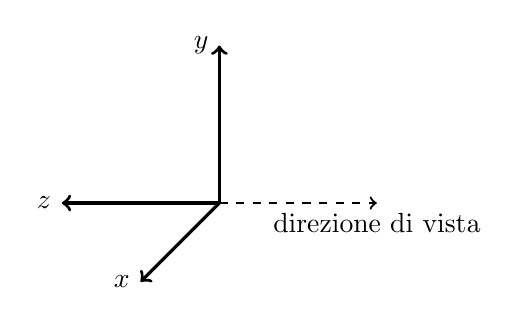
\begin{tikzpicture}[scale=2.0]
		\draw[dashed, thick, ->] (0.0, 0.0) -- (1.0, 0.0) node[below, color=black] {direzione di vista};
		\draw[very thick, ->] (0.0, 0.0) -- (-1.0, 0.0) node[left, color=black] {$z$};
		\draw[very thick, ->] (0.0, 0.0) -- (0.0, 1.0) node[left, color=black] {$y$};
		\draw[very thick, ->] (0.0, 0.0) -- (-0.5, -0.5) node[left, color=black] {$x$};
	\end{tikzpicture}
\end{center}
Questa \`e tuttavia solo una convenzione. Il vero sistema di riferimento nel quale vive la nostra scena, \`e sempre il
frame canonico. Dunque, i valori che useremo per $z$, quando trattiamo i movimenti dell'osservatore, saranno invertiti
ma poi dovranno essere svolte le opportune conversioni per rendere le modifiche consistenti con il frame canonico.

\subsection{Costruire un frame di vista (VRF)}
Un \textbf{frame di vista} o \textbf{View Reference Frame} si costruisce indicando, come prima cosa, la direzione in cui
stiamo guardando (o un punto verso cui guardare), definendo cos\`i la nostra \emph{view direction}. In seguito definiamo
qual \`e il nostro \emph{up}, ossia verso e direzione lungo i quali si sviluppa l'asse $y$.

I due assi appena definiti potrebbero non essere ortogonali fra loro per qualche motivo. Ma noi vogliamo sempre lavorare
con un frame ortonormale per evitare deformazioni indesiderate della nostra geometria.

Per ottenere un frame ortonormale dobbiamo
\begin{enumerate}
	\item Normalizzare la direzione di vista
	      \[ z = \frac{view\_direction}{\| view\_direction \|} \]
	\item Normalizzare l'\emph{up}
	      \[ y' = \frac{up}{\| up \|} \]
	\item Calcoliamo
	      \[ x = y' \times z \]
	      che sar\`a ortogonale a $z$.
	\item Calcoliamo infine
	      \[ y = x \times z \]
	      per ottenere l'asse $y$ ortogonale sia a $x$ che a $z$.
\end{enumerate}
Se scegliessimo la nostra \emph{view direction} e il nostro \emph{up}, l'uno ortogonale all'altro, ci basterebbe
calcolare il prodotto vettoriale tra i due per ottenere l'ultimo asse e costruire direttamente un frame ortogonale.

Una volta ottenuto un frame di vista ortogonale abbiamo il problema che la relativa matrice converte le coordinate dal
VRF al frame canonico quando noi vogliamo l'inverso. Per ottenere il risultato sperato ci baster\`a applicare l'inversa
\[ V = VRF^{-1} \]
che chiameremo \textbf{view matrix}.


La view matrix \`e la matrice di trasformazione che si occupa di muovere il punto di vista lungo i tre assi del VRF.

Per creare questo effetto non dobbiamo fare altro che applicare delle trasformazioni al VRF, ma pensandole in maniera
inversa.

Per esempio, se ci spostassimo verso destra, vedremo l'oggetto davanti a noi spostarsi verso sinistra.
\begin{center}
	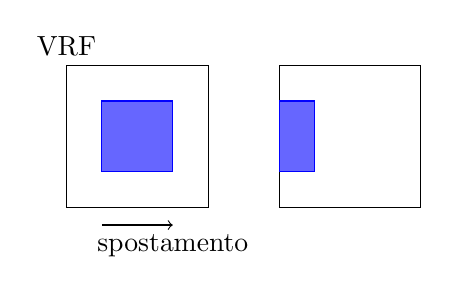
\begin{tikzpicture}[scale=0.45]
		\draw (-3, -3) --
		++ (0, 4) node[above] {VRF} --
		++ (4, 0) --
		++ (0, -4) --
		cycle;

		\draw [->] (-2, -3.5) -- ++(2, 0) node[below] {spostamento};

		\filldraw[draw=blue, fill=blue!60]
		(-2, -2) --
		++ (0, 2) --
		++ (2, 0) --
		++ (0, -2) --
		cycle;

		\draw (3, -3) --
		++ (0, 4) --
		++ (4, 0) --
		++ (0, -4) --
		cycle;

		\filldraw[draw=blue, fill=blue!60]
		(3, -2) --
		++ (0, 2) --
		++ (1, 0) --
		++ (0, -2) --
		cycle;
	\end{tikzpicture}
\end{center}
Per spostare quindi il punto di vista a destra, quello che dobbiamo fare in realt\`a, \`e spostare tutta la scena a
sinistra.

\section{Projection Matrix}
Mentre la view matrix si occupa di muovere il punto di vista nello spazio la \textbf{projection matrix} definisce il
tipo di camera che stiamo usando.

Ne esistono di due tipi, la prima \`e detta \textbf{prospettica}, la seconda invece \`e detta \textbf{ortografica}.
Questi due tipi di camera creano due effetti distinti e si prestano per compiti abbastanza differenti.

\subsection{Perspective Projection}
La \textbf{proiezione prospettica}, come suggerisce il nome, serve a creare l'effetto della prospettiva.
Con questo tipo di camera noi andremo a definire una sorta di cono visivo a partire dal punto in cui \`e posizionata
la camera.

Questo \`e il tipo di camera che ci \`e pi\`u semplice immaginare dato che funziona esattamente come l'occhio umano:
gli oggetti che si allontanano ci appaiono pi\`u piccoli e quelli che che si avvicinano ci appaiono pi\`u grandi.
Si avr\`a inoltre un effetto prospettico molto simile a quello a cui siamo abituati.
\begin{center}
	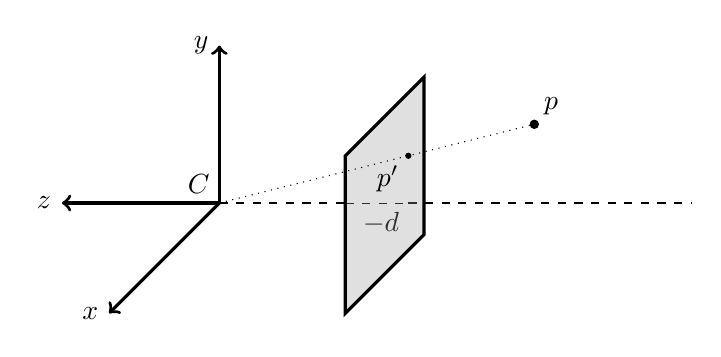
\begin{tikzpicture}[scale=2.0]
		\draw[dashed, thick] (0.0, 0.0) -- ++ (0.8, 0.0);
		\draw[dashed, ultra thin] (0.8, 0.0) -- ++ (0.4, 0.0) node[below left] {$-d$};
		\draw[dashed, thick] (1.2, 0.0) -- (3.0, 0.0);
		\draw[very thick, ->] (0.0, 0.0) -- ++ (-1.0, 0.0) node[left, color=black] {$z$};
		\draw[very thick, ->] (0.0, 0.0) -- ++ (0.0, 1.0) node[left, color=black] {$y$};
		\draw[very thick, ->] (0.0, 0.0) -- ++ (-0.7, -0.7) node[left, color=black] {$x$};

		\filldraw[very thick, fill=black!40, fill opacity=0.3]
		(0.8, 0.3) --
		++ (0, -1) --
		++ (0.5, 0.5) --
		++ (0, 1) --
		cycle;

		\coordinate (0, 0) node[above left] {$C$};

		\draw[dotted] (0.0, 0.0) -- ++ (2, 0.5);
		\fill (2, 0.5) circle[radius=0.03] node[above right] {$p$};
		\fill (1.2, 0.3) circle[radius=0.02] node[below left] {$p'$};
	\end{tikzpicture}
\end{center}
La figura rappresenta una prima parte di come funziona questo tipo di camera. In pratica dobbiamo immaginarci una
finestra (rappresentata dal quadrato grigio ad una distanza $-d$ da $C$) attraverso la quale vediamo la scena.

L'osservatore si trova nel punto $C$ e tutto ci\`o che si trova tra il punto $C$ e la finestra non viene visto. Tutto
ci\`o che invece si pu\`o osservare si trova oltre la finestra.

Il punto $p$ verr\`a proiettato sulla finestra attraverso la linea tratteggiata che lo unisce con $C$. Il punto $p'$
sar\`a appunto la proiezione del punto $p$ sulla finestra.

Per capire quali siano le coordinate di $p'$ ci conviene vedere l'immagine di lato.
\begin{center}
	\begin{tikzpicture}[scale=2.0]
		\coordinate (C) at (0, 0);
		\coordinate (p) at (2, 0.8);
		\coordinate (p1) at (1, 0.4);
		\coordinate (p_y) at (0, 0.8);
		\coordinate (p1_y) at (0, 0.4);
		\coordinate (p_z) at (2, 0);
		\coordinate (d) at (1, 0);

		% assi
		\draw[very thick, ->] (C) node[below] {$C$} -- (-1, 0) node[left] {$z$};
		\draw[thick, dashed] (C) -- (3, 0);
		\draw[very thick, ->] (C) -- (0, 1) node[above] {$y$};

		% proiezioni
		\draw[dotted] (p_y) node[left] {$p_y$} -- (p) node[above right] {$p$};
		\draw[dotted] (p1_y) node[left] {$p'_y$} -- ++ (1, 0) node[above left] {$p'$};
		\draw[dotted] (C) -- (p);
		\draw (1, -0.4) -- (d) node[below left] {$-d$} node[below right] {$p'_z$} -- ++ (0, 1.3);
		\draw[dotted] (p) -- (p_z) node[below] {$p_z$};

		\filldraw (p) circle[radius=0.035];
		\filldraw (p1) circle[radius=0.02];
	\end{tikzpicture}
\end{center}
Se notiamo, i due triangoli $C p' p'_z$ e $C p p_z$, sono simili. Questo significa che hanno gli stessi angoli interni
e che il rapporto tra i lati \`e lo stesso.

Possiamo sfruttare questo fatto per trovare le coordinate di $p'$, sapendo quelle di $p$, con una semplice proporzione
\[ p'_y : -d = p_y : p_z \]
da qui ricaviamo che
\[ p'_y = -\frac{p_y}{p_z / d} \quad p'_x = -\frac{p_x}{p_z / d} \]
mentre invece $p'_z$ e $-d$ si equivalgono.

Tutti i punti che si trovano sulla linea che va da $C$ a $p$ e che prosegue oltre $p$ verranno proiettati in $p'$.
Se esprimiamo $p'$ in coordinate omogenee
\[
	\begin{bmatrix}
		x & y & z & 1
	\end{bmatrix}
\]
Possiamo dire che qualsiasi punto di coordinate
\[
	\begin{bmatrix}
		\lambda x & \lambda y & \lambda z & \lambda
	\end{bmatrix}
\]
con $\lambda \neq 0$ verr\`a proiettato nel punto $p'$ della finestra. Volendo possiamo riscrivere le coordinate di $p'$
in questo modo
\[
	p' = \begin{bmatrix}
		-\displaystyle\frac{p_x}{p_z / d} &
		-\displaystyle\frac{p_y}{p_z / d} &
		-d                                &
		1
	\end{bmatrix}
\]
Per una ragione che analizzeremo tra poco ci conviene invece scrivere le coordinate del punto in questo modo:
\[
	p' = -\frac{p_z}{d}\begin{bmatrix}
		-\displaystyle\frac{p_x}{p_z / d} \\
		-\displaystyle\frac{p_y}{p_z / d} \\
		-d                                \\
		1
	\end{bmatrix} =
	\begin{bmatrix}
		p_x \\ p_y \\ p_z \\ -p_z / d
	\end{bmatrix}
\]
Se adesso consideriamo un punto nello spazio tridimensionale e lo moltiplichiamo per questa matrice
\[
	\begin{bmatrix}
		d & 0 & 0  & 0 \\
		0 & d & 0  & 0 \\
		0 & 0 & d  & 1 \\
		0 & 0 & -1 & 0
	\end{bmatrix}
\]
otteniamo le coordinate del punto $p'$ nella forma descritta poco fa
\[
	p' = \begin{bmatrix}
		d & 0 & 0  & 0 \\
		0 & d & 0  & 0 \\
		0 & 0 & d  & 1 \\
		0 & 0 & -1 & 0
	\end{bmatrix}
	\begin{bmatrix}
		p_x \\ p_y \\ p_z \\ 1
	\end{bmatrix} =
	\begin{bmatrix}
		d p_x \\ d p_y \\ d p_z \\ -p_z
	\end{bmatrix} =
	\begin{bmatrix}
		-\frac{p_x}{p_z / d} \\
		-\frac{p_y}{p_z / d} \\
		-d                   \\
		1
	\end{bmatrix}
\]
Ora possiamo trovare le coordinate del punto $p$, proiettato sulla finestra ad una distanza $-d$, semplicemente
moltiplicando la matrice per $p$.

Al variare di $d$ varia anche quanto vediamo della scena. Se $d$ \`e piccolo vedremo molto di pi\`u poich\'e saremo
pi\`u vicini alla finestra, viceversa, per valori grandi di $d$ vedremo di meno.

\subsubsection{Volume di vista}
Ora vogliamo definire il \textbf{volume di vista} entro il quale la nostra geometria viene renderizzata. Tutti i punti
fuori da esso vengono scartati.

Per definirlo  che, come vedremo, si tratter\`a di un tronco di piramide, abbiamo bisogno di alcuni parametri fondamentali
oltre alla distanza della finestra dall'osservatore: le \textbf{dimensioni della finestra} e la
\textbf{profondit\`a di visione}.

\subsubsection{Dimensioni della finestra}
Per definire le dimensioni della finestra vedremo due modi.

Il primo \`e quello in cui si specifica un \textbf{FOV} (\textbf{Field Of View}). In particolare definiremo un $xFOV$
e un $yFOV$, ossia due angoli i quali indicano rispettivamente l'angolo di visione orizzontale e quello verticale.
\begin{center}
	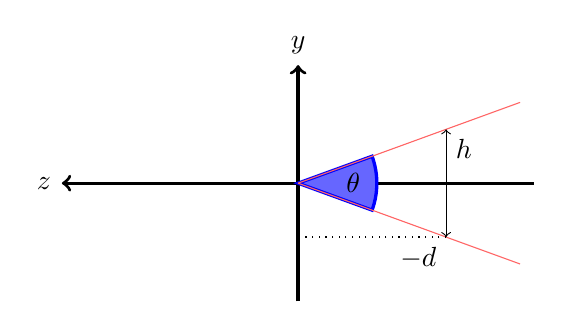
\begin{tikzpicture}
		\draw[very thick, <-] (-3, 0) node[left] {$z$} -- (3, 0);
		\draw[very thick, ->] (0, -1.5) -- (0, 1.5) node[above] {$y$};

		\filldraw[very thick, color=blue, fill=blue!60]
		(0, 0) -- (20 : 1) arc[
				start angle=20,
				end angle=-20,
				radius=1
			] -- cycle;

		\draw (0.7, 0) node {$\theta$};

		\draw[color=red!60] (0, 0) -- (20 : 3);
		\draw[color=red!60] (0, 0) -- (-20 : 3);
		\draw[<->] (20 : 2) node[below right] {$h$} -- (-20 : 2);
		\draw[dotted] (-20 : 2) node[below left] {$-d$} -- ++ (-1.9, 0);
	\end{tikzpicture}
\end{center}
L'angolo $\theta$ \`e il cosiddetto $yFOV$ e va a definire l'altezza della finestra tramite la formula
\[ h = 2d \tan{\left( \frac{yFOV}{2} \right)} \]
Ragionamento analogo per $xFOV$
\begin{center}
	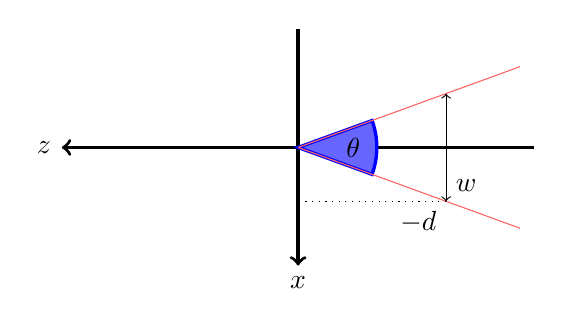
\begin{tikzpicture}
		\draw[very thick, <-] (-3, 0) node[left] {$z$} -- (3, 0);
		\draw[very thick, <-] (0, -1.5) node[below] {$x$} -- (0, 1.5);

		\filldraw[very thick, color=blue, fill=blue!60]
		(0, 0) -- (20 : 1) arc[
				start angle=20,
				end angle=-20,
				radius=1
			] -- cycle;

		\draw (0.7, 0) node {$\theta$};

		\draw[color=red!60] (0, 0) -- (20 : 3);
		\draw[color=red!60] (0, 0) -- (-20 : 3);
		\draw[<->] (20 : 2) -- (-20 : 2) node[above right] {$w$};
		\draw[dotted] (-20 : 2) node[below left] {$-d$} -- ++ (-1.9, 0);
	\end{tikzpicture}
\end{center}
L'unica cosa che cambia \`e che tramite $xFOV$ andiamo a definire
la larghezza $w$ della finestra, ottenibile allo stesso modo tramite la formula
\[ w = 2d \tan{\left( \frac{xFOV}{2} \right)} \]
Possiamo anche definire le due formule inverse per il calcolo di $xFOV$ e di $yFOV$ come segue
\begin{gather*}
	yFOV = 2 \arctan{\left( \frac{h}{2d} \right)} \\
	xFOV = 2 \arctan{\left( \frac{w}{2d} \right)}
\end{gather*}

Un altro metodo per definire le dimensioni della finestra \`e quello di specificarne i confini in maniera diretta.
\begin{center}
	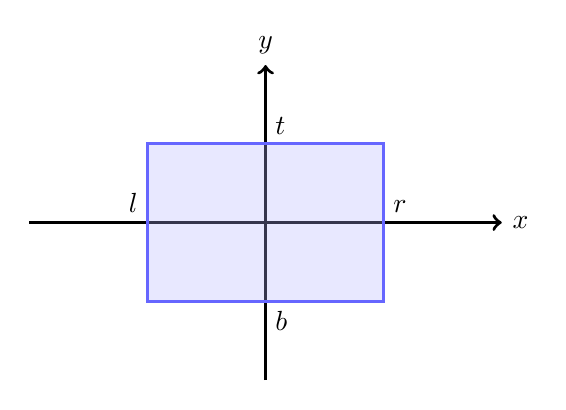
\begin{tikzpicture}
		\draw[very thick, ->] (-3, 0) -- (3, 0) node[right] {$x$};
		\draw[very thick, ->] (0, -2) -- (0, 2) node[above] {$y$};

		\draw[very thick, color=blue!60, fill=blue!30, fill opacity=0.3]
		(-1.5, 1) -- ++
		(3, 0) -- ++
		(0, -2) -- ++
		(-3, 0) --
		cycle;

		\draw (1.5, 0) node[above right] {$r$};
		\draw (-1.5, 0) node[above left] {$l$};
		\draw (0, 1) node[above right] {$t$};
		\draw (0, -1) node[below right] {$b$};
	\end{tikzpicture}
\end{center}
Come in figura andiamo a fornire quattro valori: \emph{left}, \emph{right}, \emph{top} e \emph{bottom}.
Valori che andranno a sostituire i confini del frame canonico, ossia $-1$ e $1$.

\subsubsection{Profondit\`a di visione}
Definiamo invece la profondit\`a di visione tramite due valori: \emph{near} e \emph{far}.
\begin{center}
	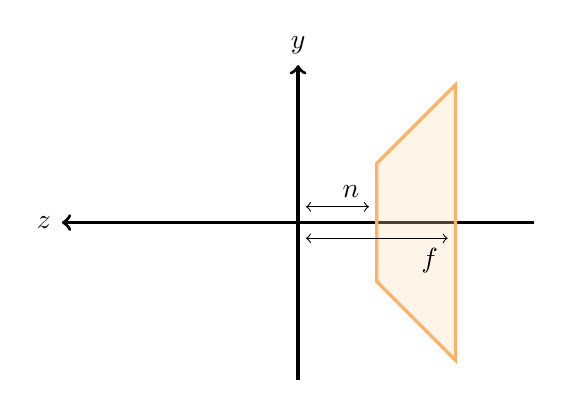
\begin{tikzpicture}
		\draw[very thick, <-] (-3, 0) node[left] {$z$} -- (3, 0);
		\draw[very thick, ->] (0, -2) -- (0, 2) node[above] {$y$};

		\draw[very thick, color=orange!60, fill=orange!30, fill opacity=0.3]
		(1, 0.75) -- ++
		(1, 1) -- ++
		(0, -3.5) -- ++
		(-1, 1) --
		cycle;

		\draw[<->] (0.1, 0.2) -- (0.9, 0.2) node[above left] {$n$};
		\draw[<->] (0.1, -0.2) -- (1.9, -0.2) node[below left] {$f$};
	\end{tikzpicture}
\end{center}
Il primo indica la distanza della finestra dall'osservatore, il secondo indica la distanza oltre il quale un punto
non viene pi\`u renderizzato dal nostro programma.

Se adesso uniamo tutto quanto ottendiamo il \textbf{volume di vista} o \textbf{view frustum}.
\begin{center}
	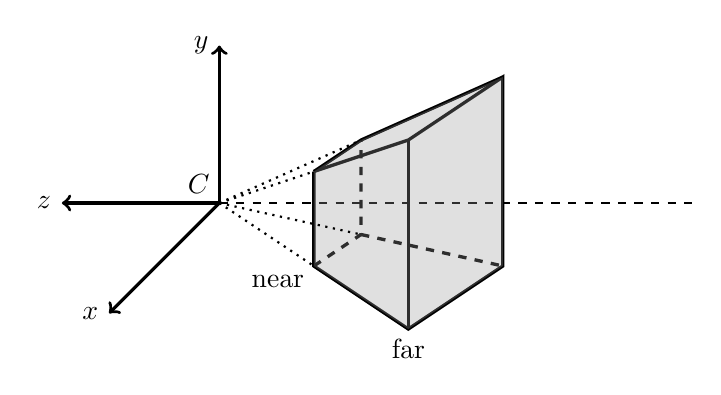
\begin{tikzpicture}[scale=2.0]
		\coordinate (n1) at (0.6, 0.2);
		\coordinate (n2) at (0.6, -0.4);
		\coordinate (n3) at (0.9, -0.2);
		\coordinate (n4) at (0.9, 0.4);

		\coordinate (f1) at (1.2, 0.4);
		\coordinate (f2) at (1.2, -0.8);
		\coordinate (f3) at (1.8, -0.4);
		\coordinate (f4) at (1.8, 0.8);

		\draw (0, 0) node[above left] {$C$};

		% assi
		\draw[very thick, ->] (0.0, 0.0) -- ++ (-1.0, 0.0) node[left, color=black] {$z$};
		\draw[dashed, thick] (0, 0.0) -- (3.0, 0.0);
		\draw[very thick, ->] (0.0, 0.0) -- ++ (0.0, 1.0) node[left, color=black] {$y$};
		\draw[very thick, ->] (0.0, 0.0) -- ++ (-0.7, -0.7) node[left, color=black] {$x$};

		\draw[very thick] (n1) -- (n2) -- (f2) -- (f3) -- (f4) -- (f1) -- (n1);
		\draw[very thick] (f1) -- (f2);
		\draw[very thick] (n1) -- (n4) -- (f4);
		\draw[very thick, dashed] (n2) -- (n3) -- (n4);
		\draw[very thick, dashed] (n3) -- (f3);

		\fill[fill=black!40, fill opacity=0.3] (n1) -- (n2) -- (f2) -- (f3) -- (f4) -- (n4) -- cycle;

		\draw[thick, dotted] (0, 0) -- (n1);
		\draw[thick, dotted] (0, 0) -- (n2);
		\draw[thick, dotted] (0, 0) -- (n3);
		\draw[thick, dotted] (0, 0) -- (n4);

		\draw (n2) node[below left] {near};
		\draw (f2) node[below] {far};
	\end{tikzpicture}
\end{center}
Possiamo adesso scrivere la \textbf{perspective projection matrix}
\[
	\begin{bmatrix}
		\frac{2n}{r - l} & 0                & \frac{r + l}{r - l}  & 0                  \\
		0                & \frac{2n}{t - b} & \frac{t + b}{t - b}  & 0                  \\
		0                & 0                & -\frac{f + n}{f - n} & -\frac{2fn}{f - n} \\
		0                & 0                & -1                   & 0
	\end{bmatrix}
\]
alla quale possiamo moltiplicare un punto (definito all'interno del volume di vista) per ottenere le sue coordinate
all'interno del frame canonico.
\[
	\begin{bmatrix}
		\frac{2n}{r - l} & 0                & \frac{r + l}{r - l}  & 0                  \\
		0                & \frac{2n}{t - b} & \frac{t + b}{t - b}  & 0                  \\
		0                & 0                & -\frac{f + n}{f - n} & -\frac{2fn}{f - n} \\
		0                & 0                & -1                   & 0
	\end{bmatrix}
	\begin{bmatrix}
		p_x \\ p_y \\ p_z \\ 1
	\end{bmatrix}
\]

\subsection{Orthograpic Projection}
Nella \textbf{proiezione ortografica} il nostro volume di vista non sar\`a pi\`u un tronco di piramide ma sar\`a un
parallelepipedo. Questo \`e dato dal fatto che prima consideravamo un singolo punto da cui partivano tutti i raggi
prospettici o \textbf{proiettori}.

Adesso i proiettori partiranno da un piano (parallelo al piano definito dagli assi $x$ e $y$) e sono tutti paralleli fra
loro. Il risultato \`e la perdita di prospettiva ma avremo comunque il senso di cosa sia dietro e cosa sia davanti nella
scena.
\begin{center}
	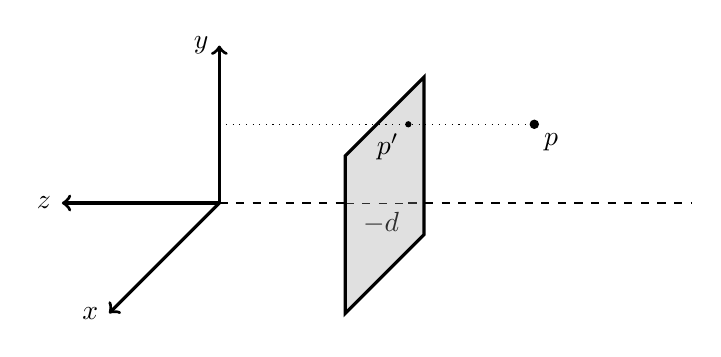
\begin{tikzpicture}[scale=2.0]
		\draw[dashed, thick] (0.0, 0.0) -- ++ (0.8, 0.0);
		\draw[dashed, ultra thin] (0.8, 0.0) -- ++ (0.4, 0.0) node[below left] {$-d$};
		\draw[dashed, thick] (1.2, 0.0) -- (3.0, 0.0);
		\draw[very thick, ->] (0.0, 0.0) -- ++ (-1.0, 0.0) node[left, color=black] {$z$};
		\draw[very thick, ->] (0.0, 0.0) -- ++ (0.0, 1.0) node[left, color=black] {$y$};
		\draw[very thick, ->] (0.0, 0.0) -- ++ (-0.7, -0.7) node[left, color=black] {$x$};

		\filldraw[very thick, fill=black!40, fill opacity=0.3]
		(0.8, 0.3) --
		++ (0, -1) --
		++ (0.5, 0.5) --
		++ (0, 1) --
		cycle;

		\draw[dotted] (0.0, .5) -- (2, 0.5);
		\fill (2, 0.5) circle[radius=0.03] node[below right] {$p$};
		\fill (1.2, 0.5) circle[radius=0.02] node[below left] {$p'$};
	\end{tikzpicture}
\end{center}
Anche in questo caso possiamo vedere come agiscono i proiettori, ma stavolta non c'\`e alcun calcolo di trigonometria
da fare per ottenere le coordinate del punto sulla finestra. Le coordinate $x, y$ specificate per il punto rimarranno
invariate sulla finestra a prescindere dal valore $z$.
\begin{center}
	\begin{tikzpicture}[scale=2.0]
		\coordinate (p) at (2, 0.8);
		\coordinate (p1) at (1, 0.8);
		\coordinate (p_y) at (0, 0.8);
		\coordinate (p_z) at (2, 0);
		\coordinate (d) at (1, 0);

		% assi
		\draw[very thick, ->] (0, 0) -- (-1, 0) node[left] {$z$};
		\draw[thick, dashed] (0, 0) -- (3, 0);
		\draw[very thick, ->] (0, 0) -- (0, 1) node[above] {$y$};

		% proiezioni
		\draw[dotted] (p_y) node[left] {$p_y$} -- (p);
		\draw (1, -0.4) -- (d) node[below left] {$-d$} node[below right] {$p'_z$} -- ++ (0, 1.3);
		\draw[dotted] (p) -- (p_z) node[below] {$p_z$};

		\filldraw (p) node[above right] {$p$} circle[radius=0.035];
		\filldraw (p1) node[above right] {$p'$} circle[radius=0.02];
	\end{tikzpicture}
\end{center}
Anche qui definiamo il nostro volume di vista in maniera del tutto analoga alla proiezione prospettica. Indichiamo quindi
i soliti sei valori: \emph{left}, \emph{right}, \emph{top}, \emph{bottom}, \emph{near} e \emph{far}.
\begin{center}
	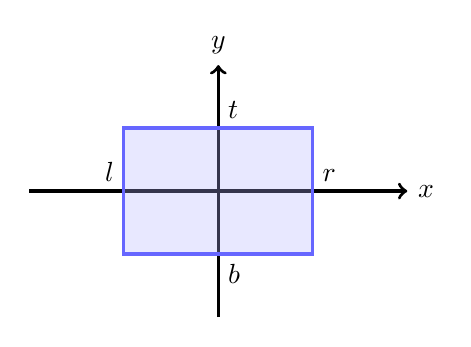
\begin{tikzpicture}[scale=0.8]
		\draw[very thick, ->] (-3, 0) -- (3, 0) node[right] {$x$};
		\draw[very thick, ->] (0, -2) -- (0, 2) node[above] {$y$};

		\draw[very thick, color=blue!60, fill=blue!30, fill opacity=0.3]
		(-1.5, 1) -- ++
		(3, 0) -- ++
		(0, -2) -- ++
		(-3, 0) --
		cycle;

		\draw (1.5, 0) node[above right] {$r$};
		\draw (-1.5, 0) node[above left] {$l$};
		\draw (0, 1) node[above right] {$t$};
		\draw (0, -1) node[below right] {$b$};
	\end{tikzpicture}
	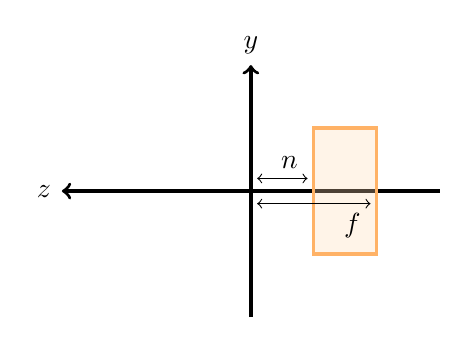
\begin{tikzpicture}[scale=0.8]
		\draw[very thick, <-] (-3, 0) node[left] {$z$} -- (3, 0);
		\draw[very thick, ->] (0, -2) -- (0, 2) node[above] {$y$};

		\filldraw[very thick, color=orange!60, fill=orange!30, fill opacity=0.3]
		(1, 1) -- ++
		(1, 0) -- ++
		(0, -2) -- ++
		(-1, 0) --
		cycle;

		\draw[<->] (0.1, 0.2) -- (0.9, 0.2) node[above left] {$n$};
		\draw[<->] (0.1, -0.2) -- (1.9, -0.2) node[below left] {$f$};
	\end{tikzpicture}
\end{center}
Otteniamo cos\`i il nostro volume di vista
\begin{center}
	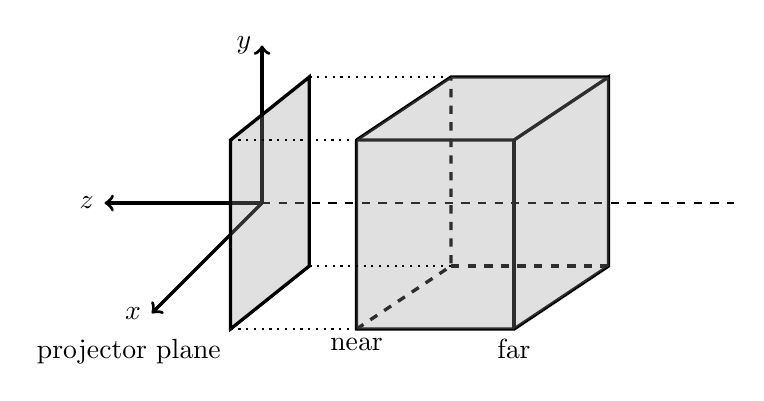
\begin{tikzpicture}[scale=2.0]
		\coordinate (n1) at (0.6, 0.4);
		\coordinate (n2) at (0.6, -0.8);
		\coordinate (n3) at (1.2, -0.4);
		\coordinate (n4) at (1.2, 0.8);

		\coordinate (f1) at (1.6, 0.4);
		\coordinate (f2) at (1.6, -0.8);
		\coordinate (f3) at (2.2, -0.4);
		\coordinate (f4) at (2.2, 0.8);

		\coordinate (p1) at (-0.2, 0.4);
		\coordinate (p2) at (-0.2, -0.8);
		\coordinate (p3) at (0.3, -0.4);
		\coordinate (p4) at (0.3, 0.8);

		% assi
		\draw[very thick, ->] (0.0, 0.0) -- ++ (-1.0, 0.0) node[left, color=black] {$z$};
		\draw[dashed, thick] (0, 0.0) -- (3.0, 0.0);
		\draw[very thick, ->] (0.0, 0.0) -- ++ (0.0, 1.0) node[left, color=black] {$y$};
		\draw[very thick, ->] (0.0, 0.0) -- ++ (-0.7, -0.7) node[left, color=black] {$x$};

		\draw[very thick] (n1) -- (n2) -- (f2) -- (f3) -- (f4) -- (f1) -- (n1);
		\draw[very thick] (f1) -- (f2);
		\draw[very thick] (n1) -- (n4) -- (f4);
		\draw[very thick, dashed] (n2) -- (n3) -- (n4);
		\draw[very thick, dashed] (n3) -- (f3);

		\fill[fill=black!40, fill opacity=0.3] (n1) -- (n2) -- (f2) -- (f3) -- (f4) -- (n4) -- cycle;

		\filldraw[very thick, fill=black!40, fill opacity=0.3] (p1) -- (p2) -- (p3) -- (p4) -- cycle;

		\draw[thick, dotted] (p1) -- (n1);
		\draw[thick, dotted] (p2) -- (n2);
		\draw[thick, dotted] (p3) -- (n3);
		\draw[thick, dotted] (p4) -- (n4);

		\draw (n2) node[below] {near};
		\draw (f2) node[below] {far};
		\draw (p2) node[below left] {projector plane};
	\end{tikzpicture}
\end{center}
La matrice relativa a questo tipo di proiezione \`e la \textbf{orthographic projection matrix} ed \`e cos\`i definita
\[
	\begin{bmatrix}
		\frac{2}{r - l} & 0               & 0                & \frac{r + l}{r - l}  \\
		0               & \frac{2}{t - b} & 0                & \frac{t + b}{t - b}  \\
		0               & 0               & -\frac{2}{f - n} & -\frac{f + n}{f - n} \\
		0               & 0               & 0                & 1
	\end{bmatrix}
\]

\section{Pipeline delle trasformazioni}
Dunque le tre principali matrici di trasformazione sono
\begin{itemize}
	\item \textbf{Model Matrix}: applica trasformazioni ad una o pi\`u figure presenti nella nostra scena.
	\item \textbf{View Matrix}: muove il punto di vista.
	\item \textbf{Projection Matrix}: delimita il volume entro cui la nostra geometria viene renderizzata.
\end{itemize}
Queste tre matrici sono uno standard e vanno sempre applicate. Sono in tutto e per tutto matrici di trasformazione e
vanno moltiplicate ai punti che compongono la scena.

Come abbiamo gi\`a detto per\`o, l'ordine con cui si effettuano le moltiplicazioni \`e importante. Per come queste
matrici sono definite in OpenGL, l'ordine \`e
\[ P \cdot V \cdot M \]
